% Auto-generated by `python new.py summarize` on 2026-06-10T10:36:21.
% Folder: experiments/2026-06-10_cka_Qwen2.5-0.5B-Instruct_qwen_mensaje/
% Paste into a beamer document. Adjust the graphicspath or paths below if compiling from a different working directory.
%
% Requires: \usepackage{graphicx}

\begin{frame}{layers --- Block CKA supermatrix at layer 12 (pooling: mean)}
  \begin{center}
    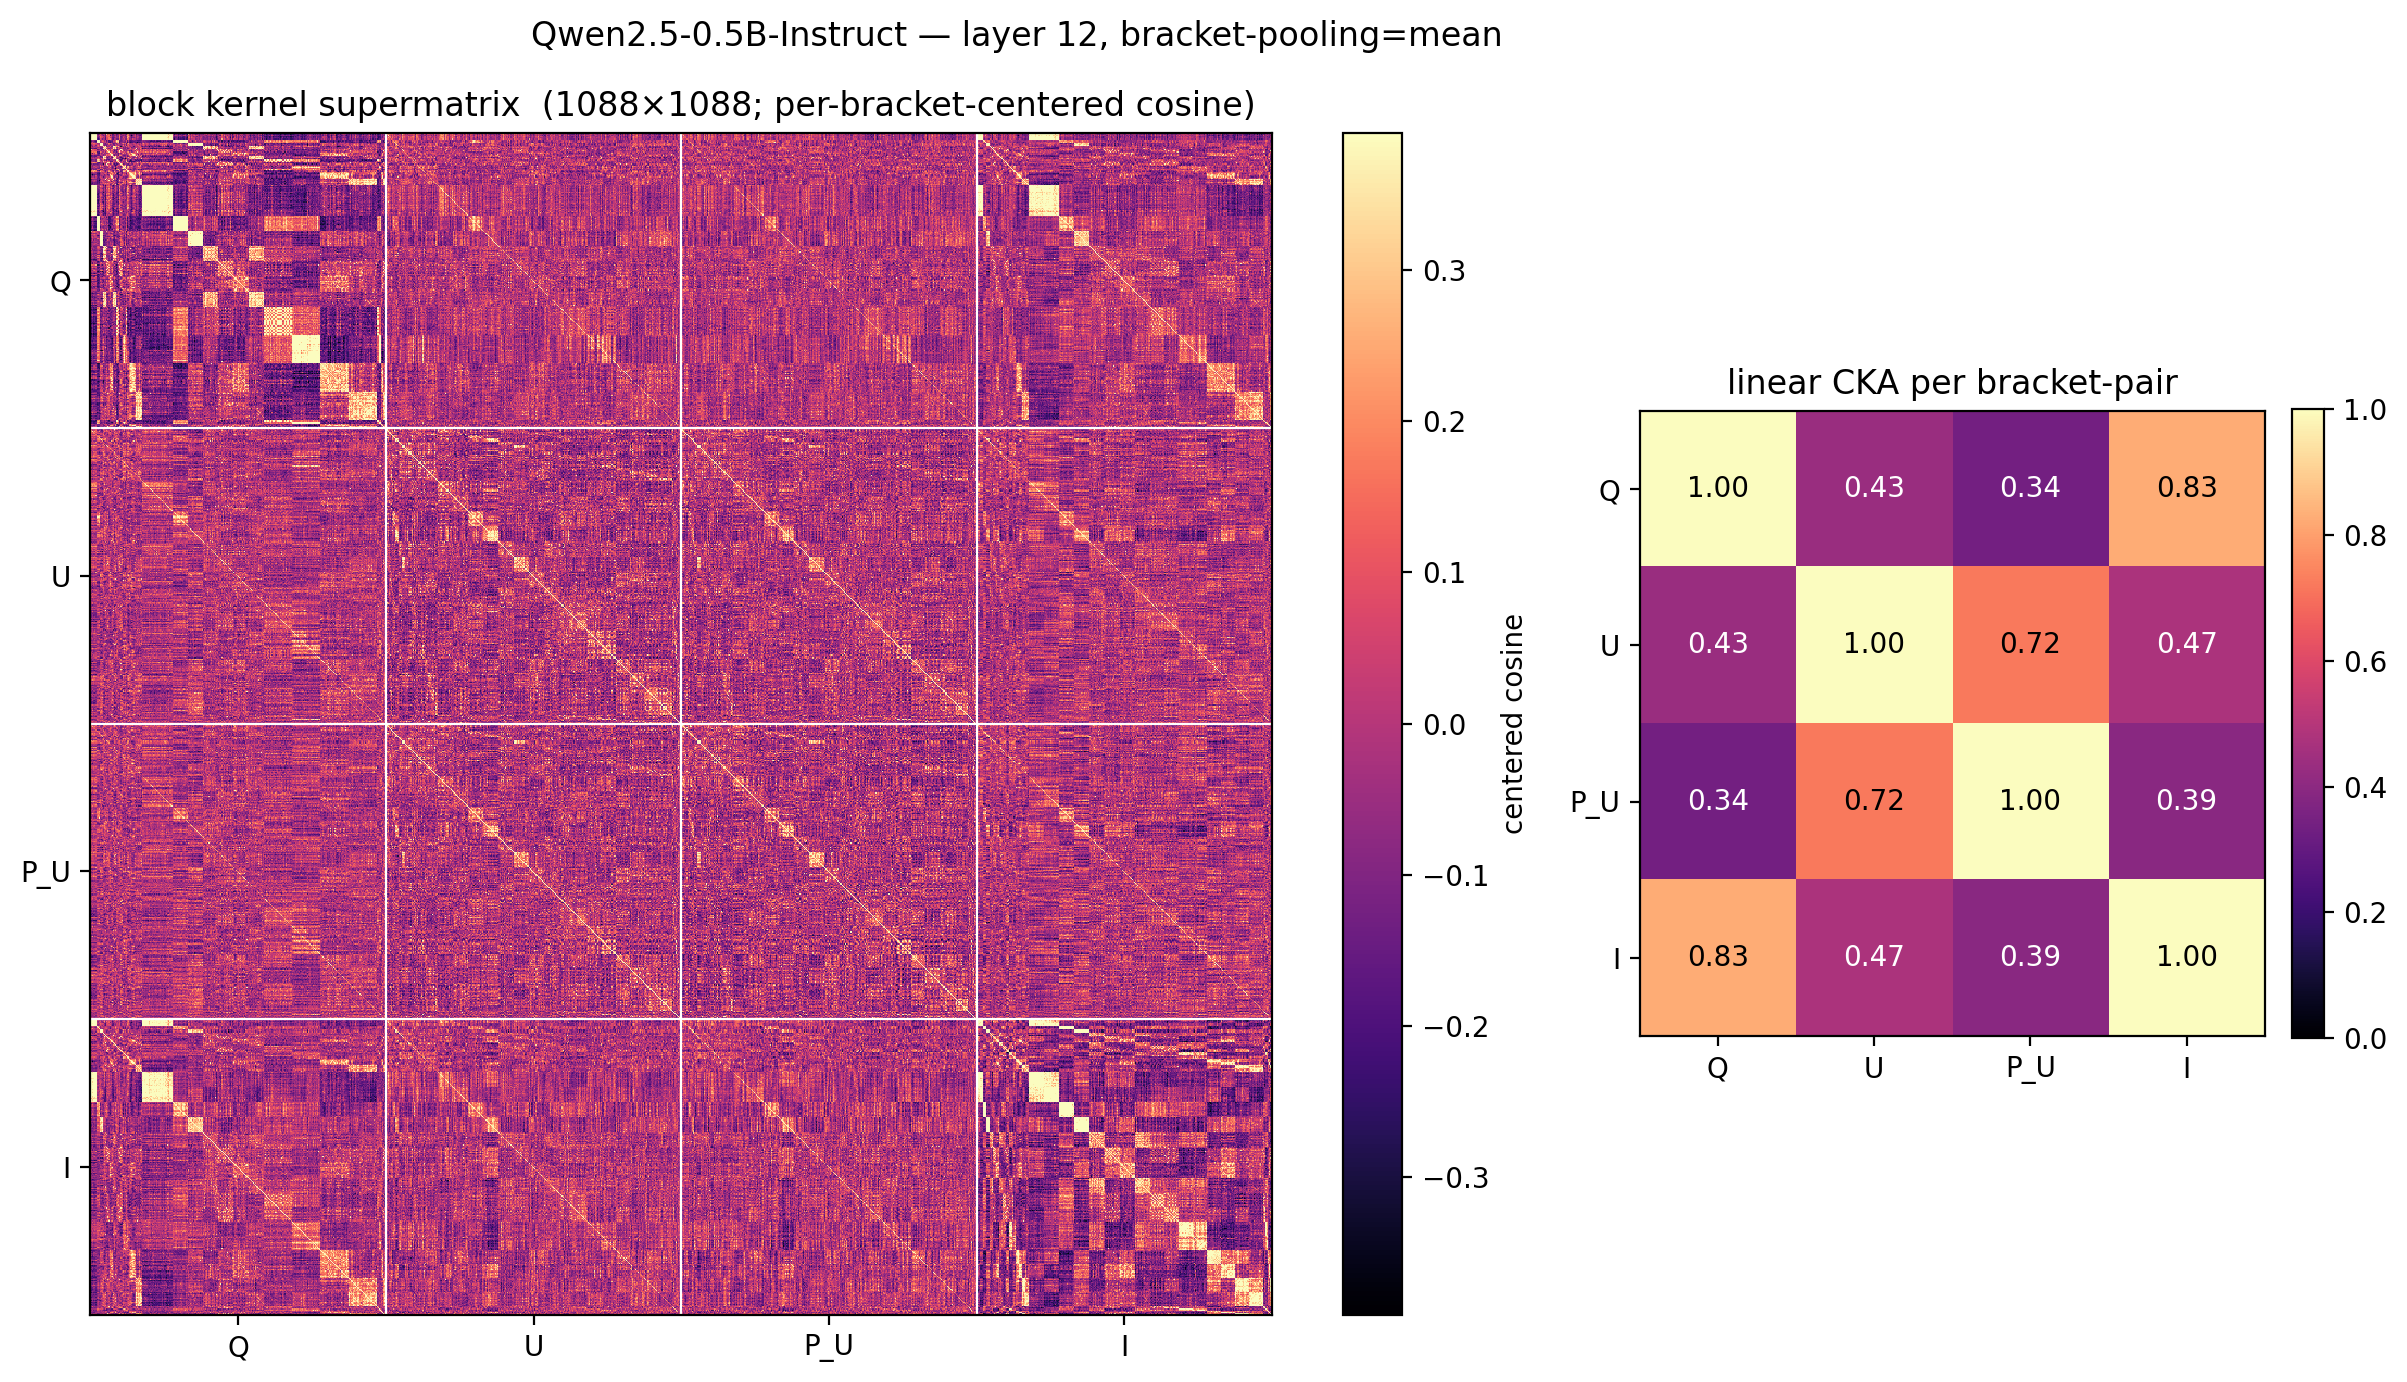
\includegraphics[width=0.95\textwidth,height=0.82\textheight,keepaspectratio]{experiments/2026-06-10_cka_Qwen2.5-0.5B-Instruct_qwen_mensaje/plots/layers/cka_blocks_L12_mean.png}
  \end{center}
\end{frame}

\begin{frame}{layers --- Block CKA supermatrix at layer 12 (pooling: mean)}
  \small
  \textbf{Computation.} At one layer, build the $(K\!\cdot\!N)\times(K\!\cdot\!N)$ centered-cosine supermatrix for all bracket pairs. Side panel: the $K\times K$ linear-CKA summary.
  \par\vspace{0.8em}
  \textbf{Interpretation.} Single-layer snapshot. Diagonal blocks are within-bracket, off-diagonals are cross-bracket. Useful for visually validating an interesting depth picked from the all-layers plot.
\end{frame}
